\chapter{Versionsmanagement}

Moderne Softwareprogrammierung wird immer komplexer, sie muss meist von mehreren Programmierern gemeinsam erledigt werden, dies erfordert einen hohen Organisationsaufwand, da jeder Programmierer nur noch einen kleinen Teil des Quellcodes erstellt und diese Teile zusammengeführt werden müssen. Ferner besteht ein System sowohl aus verschiedenen Versionen als auch Varianten, dies muss ebenfalls gemanaged werden insbesondere um „Bugs“ zu verhindern.
\\
Das Erstellen einer neuen Version bedingt durch einen Ausschneiden, Einfügen oder Löschen von bereits vorhandenem Code wird dabei \Gu history step\Go (\cite{cm_vc}, S. 41) genannt. 
Die Schrittweise Entwicklung wird durch die Versionskontrolle nachvollziehbar gemacht, da sowohl das Original als auch die Vorgängerversion für jeden \Gu history step\Go erhalten bleiben. So ist die Entwicklung auch später noch nachvollziehbar und im Gegensatz zu einem herkömmlichen Back-Up wurde mit der Prämisse gearbeitet so viel Speicherplatz wie möglich zu sparen. Dies wird durch Kompressionsverfahren ermöglicht. \cite{cm_vc}
\\
Gemäß dem ITIL-Standard umfasst Versionsmanagement „alle Verfahren von der Anforderungsbearbeitung über die Planung der Umsetzung, Tests und Abnahme von Soft- und Hardwareversionen bis hin zur organisatorischen und technischen Vorbereitung der Einführung einer Komponente“. \cite{itil_infosec}, S. 20

\section{Anfänge der Versionierung}

\textbf{SCCS (Source Code Control System)}
\\
\acs{SCCS} wurde 1972 in den Bell Labs entwickelt und wurde später in C neu geschrieben um in UNIX Systemen eingesetzt werden zu können, diese Möglichkeit wurde auch genutzt weswegen SCCS in vielen UNIX-Distributionen zur Verfügung stand. Es war bis zum Erscheinen von RCS (siehe Unten) das am Meisten genutzte System zur Versionierung. 
\\
Die Idee von SCCS war, dass eine Software \Gu linear\Go entwickelt wird, also eine neuere Version seine jeweilige Vorgängerversion ablöst, wobei die Versionen dabei nach dem Schema \Gu X.Y\Go durchnummeriert werden. Bei einer größeren Änderung wird „X“ erhöht, bei einer kleineren Änderung das „Y“. Für jeden \Gu history step\Go wird dabei um Speicherplatz zu sparen nur das \Gu Delta \Go, also die Änderung im Vergleich zur Vorgängerversion, gespeichert. Die nachfolgende Abbildung verdeutlicht dies, die Quader stehen dabei für Versionen, die Dreiecke für die jeweiligen Deltas.
\begin{figure}[H]
	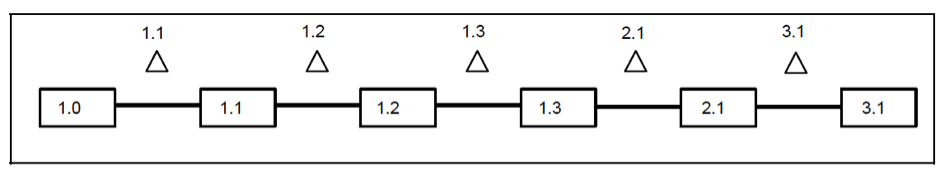
\includegraphics[width=\textwidth]{img/vcm1.png}
	\label{fig:vcm1}
	\caption{ SCCS nach \cite{cm_vc}, S. 43}
\end{figure}

Wichtig dabei ist, dass es sich um \Gu forward deltas \Go (\cite{cm_vc}, S. 43), also vorwärts gerichtete Deltas, handelt. Dies heißt, dass SCCS immer die Ursprungsversion speichert und für diese dann alle weiteren Änderungen. Die gesamte Speicherung erfolgt dabei in einer einzigen Datei und es ist auch möglich, dass eine Version zwei Nachfolger hat, jedoch nicht mehr als zwei. \cite{cm_vc}

\textbf{RCS (Revision Control System)}
\\
\acs{RCS} wurde in den 80ern als Alternative zu dem bis dahin sehr populären SCCS von Walter F. Tichy als freie Alternative zu diesem Veröffentlicht. Mit RCS wurden viele der Funktionen wie z.B. Speicherung, Logging oder das Zusammenführen von Codeteilen automatisiert und somit vereinfacht. RCS arbeitete damit hauptsächlich mit dem UNIX \textit{diff}-Kommando, das die Unterschiede zwischen zwei Dateien ermitteln kann.
\\
Wie auch \acs{SCCS} unterstützt \acs{RCS} jedoch nur eine einzelne Datei zur Speicherung des Codes und es fehlt auch die Unterstützung für komplette Projekte bzw. Ordnerstrukturen und es war Entwicklern auch nicht möglich gemeinsam an einem großen Projekt zu arbeiten.
\\
RCS war von Anfang an darauf ausgelegt, dass die Entwicklung einer Baumstruktur gleicht, also eine Version auch mehrere Nachfolgerversionen haben kann. Deswegen wird dies im Gegensatz zu SCCS auch besser unterstützt. Des Weiteren wurde in RCS auch das automatische Zusammenführen verschiedener Versionen implementiert. Dabei können Versionen von Verschiedenen Verästelungen automatisch zu einer neuen Version zusammengefasst werden und mögliche Differenzen in beiden Versionen werden Markiert und für den Programmierer sichtbar gemacht wodurch dieser manuell entscheiden kann welchen Teil des Codes er übernehmen will. Im Gegensatz zu SCCS wird in RCS auch nur die aktuellste Version gespeichert und alle anderen älteren \acs{bzw.} möglicherweise parallel erstellten Versionen sind über Deltas wiederherstellbar. Diese sind für denselben Ast rückwärts gerichtet und für eine Verästelung vorwärtsgerichtet. Ein Schema von RCS ist auf der nachfolgenden Abbildung ersichtlich. \cite{cm_vc}

\begin{figure}[H]
	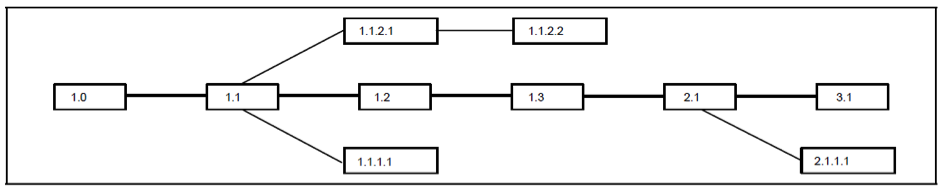
\includegraphics[width=\textwidth]{img/vcm2.png}
	\label{fig:vcm2}
	\caption {RCS nach \cite{cm_vc}, S.45}
\end{figure}

\textbf{Andere Versionierungssysteme}
\\
Natürlich sind die beiden erwähnten System (SCCS und RCS) nicht die einzigen verfügbaren Systeme. Es gibt weitere Möglichkeiten der Versionsverwaltung wie z.B. CVS oder VOODOO, auf diese soll jedoch nicht näher eingegangen werden. \cite{cm_vc}

\section{Anwendungsbeispiel - Git}
Ein verfügbares freies Programm für die Versionierung, welches heutzutage häufig genutzt wird, ist Git. Git wurde von Linus Torvalds ursprünglich für die koordinierte Entwicklung des Linux-Betriebssystems geschrieben. Im Gegensatz zu vielen anderen Tools arbeitet Git mit \Gu software revisions \Go (\cite{git_tool}, S. 1) und nicht mit Versionen die für viele Programmierer insbesondere bei Freizeitprojekten nicht von Belang sind. Stattdessen wollen diese nachvollziehen können welche Änderungen übernommen worden sind oder wie ein von ihnen geschriebener Code-Teil in das Programm eingebettet wurde.
\\
In Git werden die Dateien vergleichbar mit einem kleinen \Gu filesytem\Go (\cite{git_scm}, S.5) gespeichert, für jede Änderung wird ein Abbild der aktuellen Datenstruktur erzeugt, dies ist auf der  Abbildung \ref{fig:git} ersichtlich.
\\
Git ermöglicht es Programmierern das Komplette „Software-Repository“ zu kopieren und ihre eigenen privaten Zweige zu erstellen und zu löschen, kleine unvollständige Änderungen einzureichen oder die komplette Code-Revision zu vertagen. Ferner ermöglicht es Git den Programmierern genau festzustellen wo eine Änderung durchgeführt wurde und es behält einen kompletten Graph zur Übersicht über alle Änderungen, so müssen Sie sich nicht mit kleinen Dateien befassen in denen möglicherweise Änderungen erfolgt sind, sondern haben die Übersicht über das komplette Programm. 
\begin{figure}[H]
	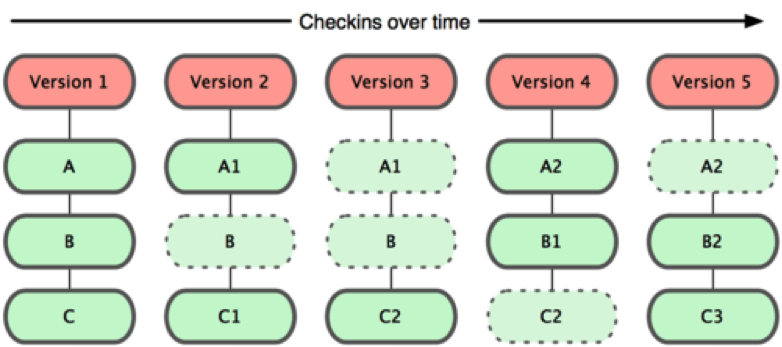
\includegraphics[width=0.9\textwidth]{img/git.png}
	\caption{Git nach \cite{git_scm}, S.5}
	\label{fig:git}
\end{figure}

Die private Kopie des Repositorys ermöglicht auch neue Arbeitsabläufe. So können Programmierer z.B. gegenseitig den Code von ihren Repositorys laden oder ein Integrations-Manager kann von jedem seiner Programmierer frei und ohne diese zu beeinflussen Code holen und diesen in das „master repository“ (\cite{git_tool}, S2) einbetten. Ferner ermöglicht es Programmierer zu entlasten, da das Coding mehrstufig aufgebaut werden kann. Dies heißt, dass vergleichbar mit der Linux-Kernel-Entwicklung zunächst die Programmierer den Code schreiben, in der nächsten Stufe wird dieser Code in Teilprojekte integriert welche dann wiederum in das Gesamt-Projekt integriert werden können.
\\
Ein weiterer Vorteil der lokalen Speicherung besteht darin, dass ein Programmierer nicht zwangsläufig Zugang zum Internet benötigt. Stattdessen kann er seine Änderungen „offline“ implementieren und zu einem Zeitpunkt seiner Wahl zum „master repository“  hinzufügen. Des Weiteren sind die Zugriffszeiten bei dieser Art der Speicherung geringer und die Produktivität sollte steigen.
\\
Git ermöglicht es zudem ein Repository für die Öffentlichkeit zur Verfügung zu stellen. Mittlerweile kann dieses auch von einem Drittanbieter wie etwa GitHub gehostet werden. Wobei der Anbieter das „repository management“ (\cite{git_tool}, S. 2) über eine Browser-Schnittstelle gewährleistet. 
\\
\cite{git_scm}, \cite{git_tool}
